\documentclass[]{article}
\usepackage{amsmath}
\usepackage{amssymb}
\usepackage{stmaryrd}
\usepackage{latexsym}
\usepackage{graphicx}
\usepackage{fancyhdr}
\usepackage{color}
\usepackage{listings}
\usepackage[top=1in, right=0.75in, left=0.75in]{geometry}
\usepackage[colorlinks=true, linkcolor=blue]{hyperref}

\definecolor{customgreen}{rgb}{0,0.6,0}
\definecolor{customgray}{rgb}{0.5,0.5,0.5}
\definecolor{custommauve}{rgb}{0.6,0,0.8}

\definecolor{dkgreen}{rgb}{0,0.6,0}
\definecolor{gray}{rgb}{0.5,0.5,0.5}
\definecolor{mauve}{rgb}{0.58,0,0.82}

\lstset{frame=tb,
	language=MATLAB,
	aboveskip=3mm,
	belowskip=3mm,
	showstringspaces=false,
	columns=flexible,
	frame=single,	                   % adds a frame around the code
	basicstyle={\small\ttfamily},
	numbers=none,
	numberstyle=\tiny\color{gray},
	keywordstyle=\color{blue},
	commentstyle=\color{dkgreen},
	stringstyle=\color{mauve},
	breaklines=true,
	rulecolor=\color{black},
	breakatwhitespace=true,
	tabsize=3,
	numbers=left,                    % where to put the line-numbers; possible values are (none, left, right)
	numbersep=10pt,                   % how far the line-numbers are from the code
	numberstyle=\tiny\color{customgray}, % the style that is used for the line-numbers
}

\author{
	Mohammad Hossein Shafizadegan\\
	99104781
}
\title{
	Coding Assignment 1 \\
	Computational Intelligence  \\
	Dr. S. Hajipour
}

\pagestyle{fancy}
\rhead{CI}
\lhead{CHW 1}

\newcommand{\pict}[2]{\begin{center}
		\includegraphics[width=#1\linewidth]{Fig/#2.png}
\end{center}}
\newcommand{\mat}[1]{\begin{bmatrix} #1 \end{bmatrix}}
\newcommand{\deter}[1]{\begin{vmatrix} #1 \end{vmatrix}}

\definecolor{customgreen}{rgb}{0,0.6,0}
\definecolor{customgray}{rgb}{0.5,0.5,0.5}
\definecolor{custommauve}{rgb}{0.6,0,0.8}

\definecolor{dkgreen}{rgb}{0,0.6,0}
\definecolor{gray}{rgb}{0.5,0.5,0.5}
\definecolor{mauve}{rgb}{0.58,0,0.82}

\lstset{frame=tb,
	language=MATLAB,
	aboveskip=3mm,
	belowskip=3mm,
	showstringspaces=false,
	columns=flexible,
	frame=single,	                   % adds a frame around the code
	basicstyle={\small\ttfamily},
	numbers=none,
	numberstyle=\tiny\color{gray},
	keywordstyle=\color{blue},
	commentstyle=\color{dkgreen},
	stringstyle=\color{mauve},
	breaklines=true,
	rulecolor=\color{black},
	breakatwhitespace=true,
	tabsize=3,
	numbers=left,                    % where to put the line-numbers; possible values are (none, left, right)
	numbersep=10pt,                   % how far the line-numbers are from the code
	numberstyle=\tiny\color{customgray}, % the style that is used for the line-numbers
}

\begin{document}
	\begin{figure}
		
\includegraphics[width=0.25\textwidth]{Fig/Sharif.png}
		\centering
	\end{figure}
	\maketitle
	\tableofcontents
	\newpage
		%-----------------------------------------------------------------------------------------------------------------	
	\section{Question 1}
	\subsection*{a}
	In order to obey clean code rules, we have a developed a function called "plot\_fact" for this section. The initial values of the parameters will be provided to this function as input arguments.
	\begin{lstlisting}
		function plot_fact(init_w1, init_w2, init_T, beta)
	\end{lstlisting}
	 In this function, we have to define and create a \textit{meshgrid} for $X$ and $Y$ as follows:
	\begin{lstlisting}
		global p % define a global variable for the plot handle
		dx = 0.01;
		dy = 0.01;
		beta = 0.5;
		
		x = -1:dx:1;
		y = -1:dy:1;
		[X,Y] = meshgrid(x,y);
	\end{lstlisting}
	Then we assign random initial values to $w_1$, $w_2$, and $T$ and form the activation function.
	\begin{lstlisting}
		% initialize some initial values for w1, w2, and T
		w1 = 0.5;
		w2 = 0.5;
		T = 0.5;
		
		f_act = 1./(1 + exp(-1*beta.*(w1*X+w2*Y-T))); % calculate the initial f_act values
	\end{lstlisting}
	After that we have to deal with interactive sliders for each of the parameters. Using MATLAB builtin \textit{uicontrol} command, we create three sliders. The code used for creating one of these sliders can be seen below.
	\begin{lstlisting}
		% Slide bar for w1
		s_w1 = uicontrol('Parent',f,'Style','slider','Position',[81,110,419,23],...
									   'value',w1, 'min',-5, 'max',5);
		bgcolor = f.Color;
		sl1 = uicontrol('Parent',f,'Style','text','Position',[50,110,23,23],...
								   'String','-5','BackgroundColor',bgcolor);
		sl2 = uicontrol('Parent',f,'Style','text','Position',[500,110,23,23],...
								   'String','5','BackgroundColor',bgcolor);
		sl3 = uicontrol('Parent',f,'Style','text','Position',[240,85,100,23],...
								   'String','w1','BackgroundColor',bgcolor);
	\end{lstlisting}
	In order to interactively change the parameters and observe the results, we have to develop a callback function for the sliders and assign the callback function to them. In the callback function, we first parse the new value of the parameters, then we generate the activation function again regarding new values. The code for the callback function is as follows:
	\begin{lstlisting}
		function update (src, event, b_w1, b_w2, b_T)
			global p % access the global variable p
			dx = 0.01;
			dy = 0.01;
			beta = 0.5;
			
			x = -1:dx:1;
			y = -1:dy:1;
			[X,Y] = meshgrid(x,y);
			
			w1 = get(b_w1, 'Value'); % get the current slider value for w1 using the get function
			w2 = get(b_w2, 'Value'); % get the current slider value for w2 using the get function
			T = get(b_T, 'Value'); % get the current slider value for T using the get function
			f_act = 1./(1 + exp(-1*beta.*(w1*X+w2*Y-T))); % calculate the new f_act values
			p.ZData = f_act; % update the plot 
			
			fprintf("w1= %d   ,   w2 = %d   ,   T = %d \n", w1, w2, T);
			
		end
	\end{lstlisting}
	The result can be seen below:
	\pict{0.5}{Q1_F1}
	
	\subsection*{b}
	Here we simply set $w_1=w_2=T=\beta=1$. The results will be as follows:
	\begin{center}
		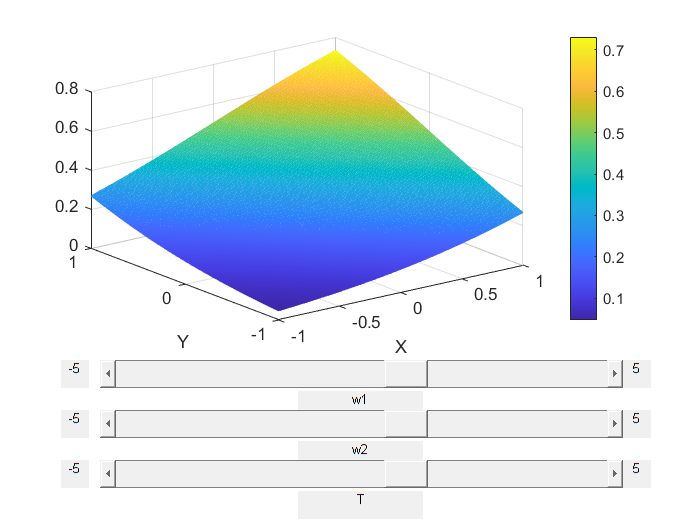
\includegraphics[width=0.4\linewidth]{Fig/Q1_F2.png}
		\qquad\qquad
		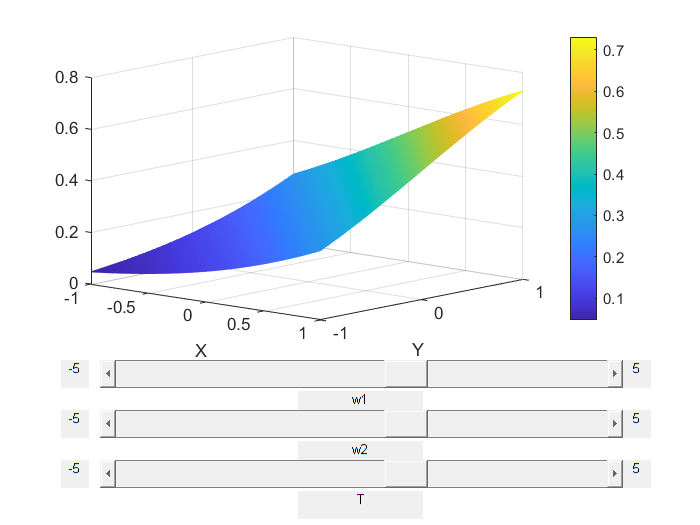
\includegraphics[width=0.4\linewidth]{Fig/Q1_F3.png}
	\end{center}

	\subsection*{c}
	In order to implement the OR function, we have to set the value of each weights equal to 2 and the threshold will be 1. As it is said in the instructions, we choose a huge value for $\beta$, e.g. 100.
	\begin{lstlisting}
		%% part C
		
		% OR function
		w1 = 2;
		w2 = 2;
		T = 1;
		
		beta = 100;
		
		plot_fact(w1, w2, T, beta)
	\end{lstlisting}
	The results can be seen here.
	\begin{center}
		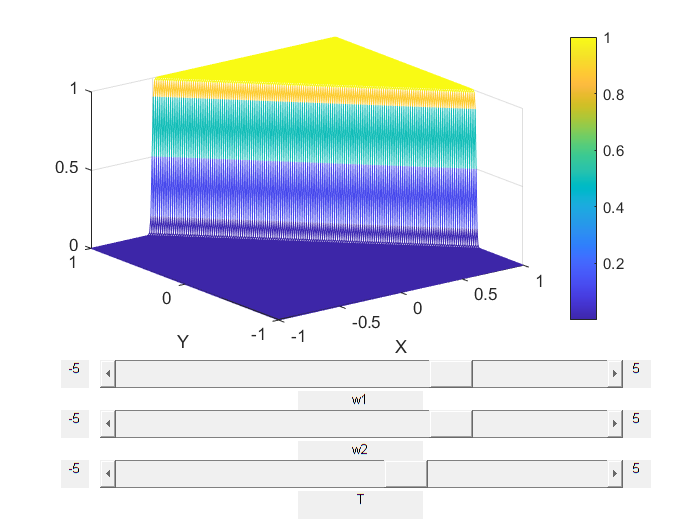
\includegraphics[width=0.4\linewidth]{Fig/Q1_F4.png}
		\qquad\qquad
		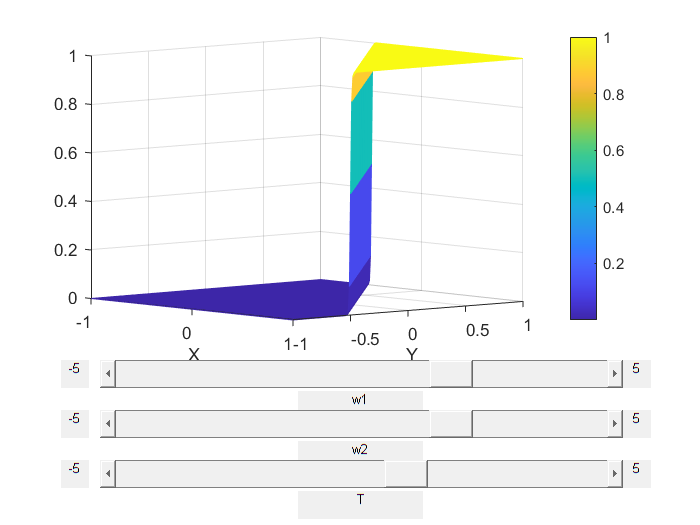
\includegraphics[width=0.4\linewidth]{Fig/Q1_F5.png}
	\end{center}
	Based on the above figures, it can be concluded that the activation function for huge values of $\beta$ is quite the same as step threshold function.
	
	\subsection*{d}
	Now we set the value of $\beta$ to 0.1 and visualize the results.
	\pict{0.5}{Q1_F6}
	
	\section{Question 2}
	\subsection*{a}
	First we properly load the dataset into the MATLAB workspace. Then we separate the data corresponding to the first two classes after extracting their indices. The code for this section is as follows:
	\begin{lstlisting}
		% load dataset
		irisTable = readtable('../iris.csv');
		irisData = table2array(irisTable(:,1:4));
		
		% Extract data for Iris-setosa and Iris-versicolor classes
		setosa_idx = find(strcmp(irisTable.Var5, 'Iris-setosa'));
		versicolor_idx = find(strcmp(irisTable.Var5, 'Iris-versicolor'));
		
		setosa_data = irisData(setosa_idx, :);
		versicolor_data = irisData(versicolor_idx, :);
	\end{lstlisting}
	For visualizing our data in the features domain, we have developed a function named "scatter\_features" which receives data corresponding to each class and the number of two desired features as input argument. In this function, we simply visualize data using "scatter" function as follows:
	\begin{lstlisting}
		function scatter_features(data1, data2, f1,f2)
			% Plotting features: sepal length vs sepal width
			scatter(data1(:,f1), data1(:,f2), 'filled', 'MarkerFaceColor', 'r');
			hold on;
			scatter(data2(:,f1), data2(:,f2), 'filled', 'MarkerFaceColor', 'g');
			xlabel(sprintf('feature %d', f1));
			ylabel(sprintf('feature %d', f2));
			title(sprintf('feature %d vs. feature %d', f1, f2));
			legend('Iris-setosa', 'Iris-versicolor');
			hold off;
		end
	\end{lstlisting}
	Now for different combinations of features, we visualize our data to inspect which features separate our data of two classes better.
	\pict{0.9}{Q2_F1}
	Regarding this figure, we can infer that these two classes of data can be separated quite well using features 3 and 4. For the rest of this question we will use these features for training process.
	
	\subsection*{b}
	
	
	\subsection*{c}
	First we randomly separate 80\% of our data for training and their corresponding labels, as follows:
	\begin{lstlisting}
		P = randperm (50);
		train_data = [setosa_data(P(1:40), 3:4) ; versicolor_data(P(1:40), 3:4)];
		
		% all data labels within an array (first class 1 then class 0)
		out = [ones(1,40), zeros(1,40)];
	\end{lstlisting}
	In order to implement the online learning algorithm we have developed a function called "online\_learning". The input arguments of this function are the learning rate $\eta$, number of iterations, training data and their labels.\\
	This function will find the values of weights and threshold and will return these values alongside with the number of iterations actually took for achieving the convergence.
	\begin{lstlisting}
		function [w_array, theta_array, iter_num] = online_learning(eta, n_iter, x, out)
	\end{lstlisting}
	In this function, we first randomly initiate the values of the parameters. Then we have defined two matrices to store the values of weights and threshold for each iteration.
	\begin{lstlisting}
		init_w = [0; 0];
		init_theta = 5;
		
		w = init_w;
		theta = init_theta;
		
		w_array = [w];
		theta_array = [theta];
	\end{lstlisting}
	The main part of the algorithm will be discussed here as in a nested for loop, we update the values of the weights and threshold after each iteration using the delta rule. Any further explanation are provided within the code using comments. The code for this section will be as follows:
	\begin{lstlisting}
		for i = 1:n_iter
			e = 0;
			for j = 1:length(x)
				% Compute the output of the threshold logic unit (TLU)
				y = w' * x(j,:)' >= theta;
				
				% Check if the output is different from the target
				if y ~= out(j)
					% Update the threshold and store its value
					theta = theta - eta * (out(j) - y);
					theta_array = [theta_array theta];
					
					% Update the weights and store their values
					w = w + eta * (out(j) - y) * x(j,:)';
					w_array = [w_array w];
					
					% Update the error count
					e = e + abs(out(j) - y);
				end
			end
			
			% Check if the error count is less than or equal to zero
			% If true, exit the loop as the training is complete
			if e <= 0
				break;
			end
		end
	\end{lstlisting}
	Now we run this online algorithm and the final values for the weight and the threshold can be seen below.
	\begin{lstlisting}
		[w_online, theta_online, iter_num] = online_learning(eta, n_iter, train_data, out);
		
		disp('Online learning');
		fprintf('number of iterations: %d \n', iter_num)
		fprintf('the resulting weigths: w1=%d , w2=%d \n', w_online(1, end), w_online(2, end));
		fprintf('threshold = %d \n', theta_online(end));
	\end{lstlisting}
	\pict{1}{Q2_F2}
	In order to plot the achieved line, we have developed a function called "plot\_line". The code for this simple function is as follows:
	\begin{lstlisting}
		function plot_line(w1, w2, theta)
			slope = -w1/w2;
			intercept = theta/w2;
			x = 0:0.1:5;
			y = slope*x + intercept;
			plot(x,y,'r'); xlabel('x'); ylabel('y');
		end
	\end{lstlisting}
	Using this function, we visualize the results:
	\pict{0.45}{Q2_F3}
	Now for implementing the batch learning algorithm, we also develop a function called "batch\_learning". The attitude toward developing the this function is quite the same as before except for the algorithm for updating the wights and the threshold which obey the batch learning rule.\\
	The code used for updating the parameters can be seen below:
	\begin{lstlisting}
		for i = 1:n_iter
			e = 0;
			theta_c = 0;
			w_c = zeros(2,1);
			
			for j = 1:length(x)
				% Compute the output of the threshold logic unit (TLU)
				y = w' * x(j,:)' >= theta;
				
				% Check if the output is different from the target
				if y ~= out(j)
					% Update the temporary threshold and weights
					theta_c = theta_c - eta * (out(j) - y);
					w_c = w_c + eta * (out(j) - y) * x(j,:)';
					
					% Update the error count
					e = e + abs(out(j) - y);
				end
			end
			
			% Update the threshold and weights using the temporary values
			theta = theta + theta_c;
			theta_array = [theta_array theta];
			w = w + w_c;
			w_array = [w_array w];
			
			% Check if the error count is less than or equal to zero
			% If true, exit the loop as the training is complete
			if e <= 0
				break;
			end
		end
	\end{lstlisting}
	Now we run this algorithm for our data:
	\begin{lstlisting}
		[w_batch, theta_batch, n_iter_batch] = batch_learning(eta, n_iter, train_data, out);
		
		disp('Batch learning');
		fprintf('number of iterations: %d \n', n_iter_batch)
		fprintf('the resulting weigths: w1=%d , w2=%d \n', w_batch(1, end), w_batch(2, end));
		fprintf('threshold = %d \n', theta_batch(end));
	\end{lstlisting}
	\pict{1}{Q2_F5}
	Here we have visualized the results:
	\begin{lstlisting}
		figure;
		scatter_features(setosa_data, versicolor_data, 3,4); hold on;
		title('Batch learning')
		plot_line(w_batch(1, end), w_batch(2, end), theta_batch(end)); hold off;
	\end{lstlisting}
	\pict{0.6}{Q2_F4}
	
	\subsection*{d}
	Now using the matrices we define for storing the values of weights and threshold for each algorithm, we simply plot the process using subplots. Here are the codes of these sections:
	\begin{lstlisting}
		figure;
		subplot(3,1,1)
		plot(w_online(1,:))
		title('Online learning')
		xlabel('iteration')
		ylabel('w1');
		subplot(3,1,2)
		plot(w_online(2,:))
		xlabel('iteration')
		ylabel('w2');
		subplot(3,1,3)
		plot(theta_online)
		xlabel('iteration')
		ylabel('theta');
	\end{lstlisting}
	\begin{center}
		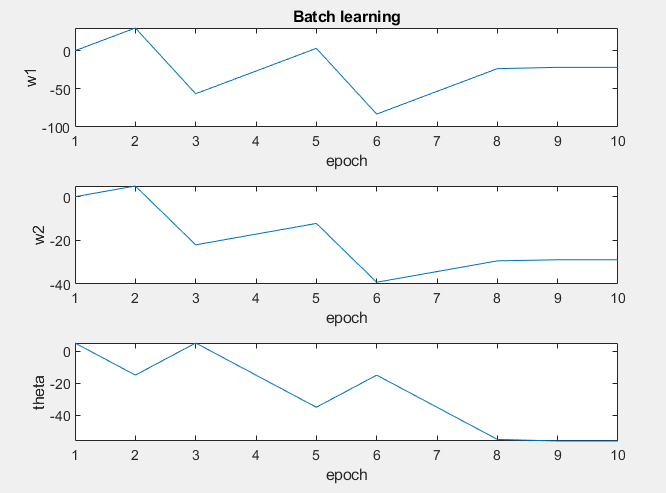
\includegraphics[width=0.4\linewidth]{Fig/Q2_F6.png}
		\qquad\qquad
		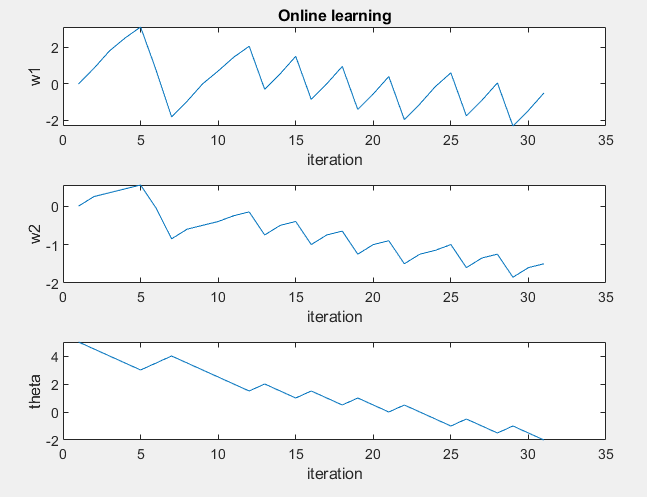
\includegraphics[width=0.4\linewidth]{Fig/Q2_F7.png}
	\end{center}

	\subsection*{e}
	As we discussed the results before, we once again demonstrate them here:
	\begin{center}
		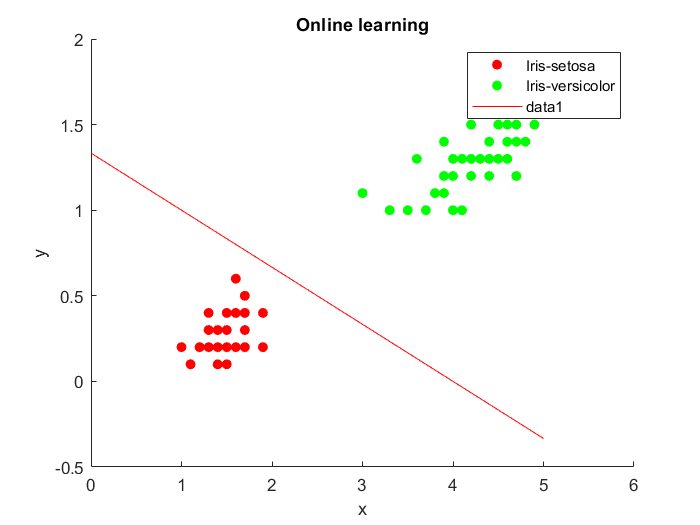
\includegraphics[width=0.3\linewidth]{Fig/Q2_F3.png}
		\qquad\qquad
		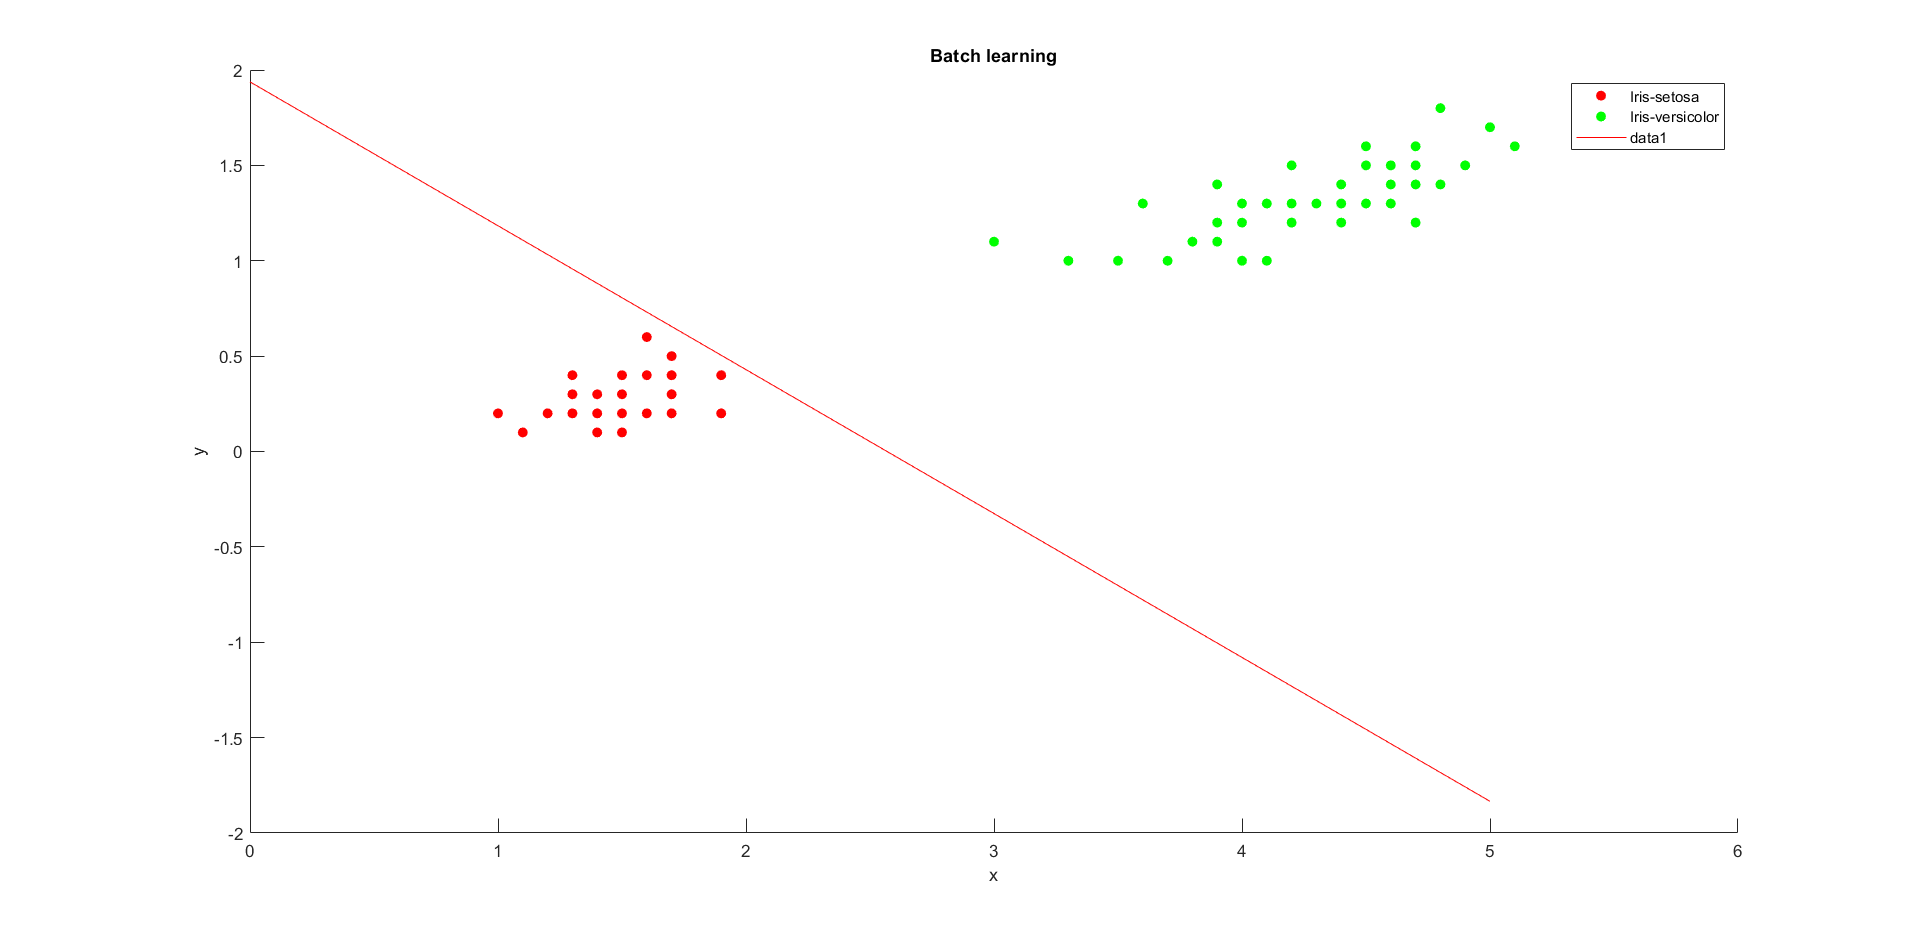
\includegraphics[width=0.5\linewidth]{Fig/Q2_F4.png}
	\end{center}

	\subsection*{f}
	In this section, we use our model for the remaining test data using this code:
	\begin{lstlisting}
		test_data = [setosa_data(P(41:50), 3:4) ; versicolor_data(P(41:50), 3:4)];
		out_test = [ones(1,10), zeros(1,10)];
		
		y_online = w_online(:, end)' * test_data' >= theta_online(end);
		
		y_batch = w_batch(:, end)' * test_data' >= theta_batch(end);
		
		acc_online = sum(y_online == out_test)/length(out_test) * 100;
		acc_batch = sum(y_batch == out_test)/length(out_test) * 100;
		
		fprintf('Accuracy of classification train by online learning: %d  \n', acc_online);
		fprintf('Accuracy of classification train by batch learning: %d \n', acc_batch);
	\end{lstlisting}
	\pict{1}{Q2_F8}
	
	\subsection*{g}
	First of all we extract data of all three classes the same way we did before. 
	\begin{lstlisting}
		% Extract data for Iris-setosa and Iris-versicolor classes
		setosa_idx = find(strcmp(irisTable.Var5, 'Iris-setosa'));
		versicolor_idx = find(strcmp(irisTable.Var5, 'Iris-versicolor'));
		virginica_idx = find(strcmp(irisTable.Var5, 'Iris-virginica'));
		
		setosa_data = irisData(setosa_idx, :);
		versicolor_data = irisData(versicolor_idx, :);
		virginica_data = irisData(virginica_idx, :);
	\end{lstlisting}
	For this section, we have modified the code for "scatter\_features" in a way to support three classes of data and three features. The result will be a 3D scatter plot with different color for each class. The main modified parts of the "scatter\_features" function can be seen below
	\begin{lstlisting}
		scatter3(data1(:,f1), data1(:,f2), data1(:,f3), 'filled', 'MarkerFaceColor', 'r');
		hold on;
		scatter3(data2(:,f1), data2(:,f2), data2(:,f3), 'filled', 'MarkerFaceColor', 'g');
		scatter3(data3(:,f1), data3(:,f2), data3(:,f3), 'filled', 'MarkerFaceColor', 'b');
	\end{lstlisting}

	For observing our dataset in the features space, we have visualized them for different combinations of features. 
	\begin{lstlisting}
		subplot(2,2,1);
		scatter_features(setosa_data, versicolor_data, virginica_data, 1, 2, 3);
		subplot(2,2,2);
		scatter_features(setosa_data, versicolor_data, virginica_data, 1, 2, 4);
		subplot(2,2,3);
		scatter_features(setosa_data, versicolor_data, virginica_data, 2, 3, 4);
		subplot(2,2,4);
		scatter_features(setosa_data, versicolor_data, virginica_data, 1, 3, 4);
	\end{lstlisting}
	The results are as follows:
	\pict{1}{Q2_F9}
	It can be seen vividly that data from classes "iris-versicolor" and "iris-virginica" can't be separated linearly using a plane. These classes are somehow a little mixed with each other which make it impossible to separate them linearly. Therefor, we can't classify these classes using a network of TLUs.\\\\
	These classes can't be separated via a single TLU obviously. Also as we discussed above, we can't even separate them using a network of TLUs with a 100\% accuracy.\\\\
	In the following we try to separate class 1 (red) and class 2 (green) using a TLU. Then we attempt to do the same for class 2 (green) and class 3 (blue). The resulting planes will divide the 3D space into three sections each for a class. The outputs of these 2 TLUs can be used by TLUs of the next layer which implements AND function and the results will be used by the output neuron to clarify the final output by binary encoding.\\\\
	Regarding the features figure, we have decided to choose features 1, 3, and 4 for classification.\\\\
	First we train a TLU for separating class 1 and class 2 using 80\% of data as training data via the following code. Also we have calculated the accuracy on the train data and test data correspondingly to assess the performance of the classifier.
	\begin{lstlisting}
		selected_features = [1, 3, 4];
		
		P = randperm (50);
		train_data = [setosa_data(P(1:40), selected_features) ; ...
		versicolor_data(P(1:40), selected_features)];
		
		% all data labels within an array (first class 1 then class 0)
		out = [ones(1,40), zeros(1,40)];
		
		n_iter = 100;
		eta = 0.5;
		
		[w_12, theta_12, iter_num] = online_learning([0; 0; 0], 0, eta, n_iter, train_data, out);
		
	\end{lstlisting}
	There results for this section can be seen below:
	\pict{1}{Q2_F10}
	\begin{center}
		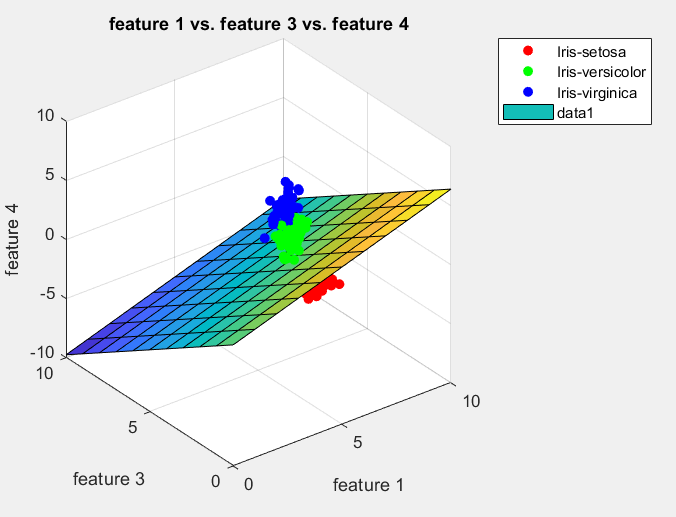
\includegraphics[width=0.4\linewidth]{Fig/Q2_F11.png}
		\qquad\qquad
		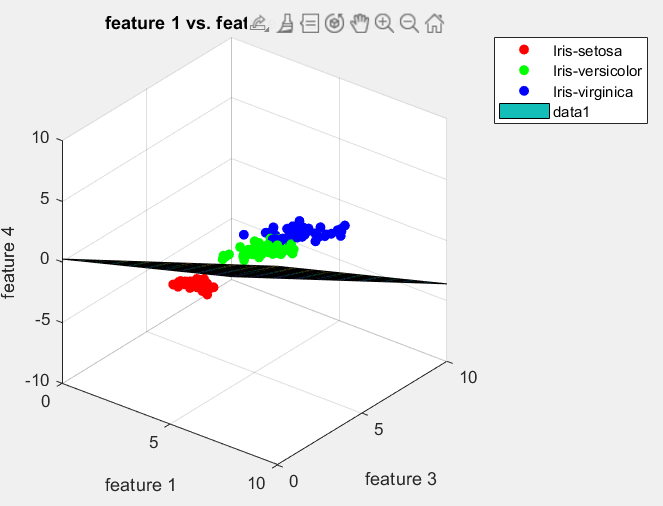
\includegraphics[width=0.4\linewidth]{Fig/Q2_F12.png}
	\end{center}
	We note that we have converted the function "plt\_line" to "plot\_plane" to support plotting a plane in 3D space.\\
	It can be seen that we can properly separate these two classes using a single TLU.\\\\
	Now we try to separate class 2 and 3 using a TLU using the same procedure.
	\begin{lstlisting}
		%% train a TLU for separating class 2 and class 3
		
		P = randperm (50);
		train_data = [versicolor_data(P(1:40), selected_features) ; ...
		virginica_data(P(1:40), selected_features)];
		
		% all data labels within an array (first class 1 then class 0)
		out = [ones(1,40), zeros(1,40)];
		
		eta = 0.01;
		n_iter = 1000;
		
		[w_23, theta_23, n_iter_23] = online_learning([0; 0; 0], 0, eta, n_iter, train_data, out);
	\end{lstlisting}
	As discussed before, we are not expecting to completely separate these data via a TLU so we have to be more careful here by choosing a smaller value for $\eta$ and increasing the number of iteration.\\
	The results are as follows:
	\pict{1}{Q2_F15}
	\begin{center}
		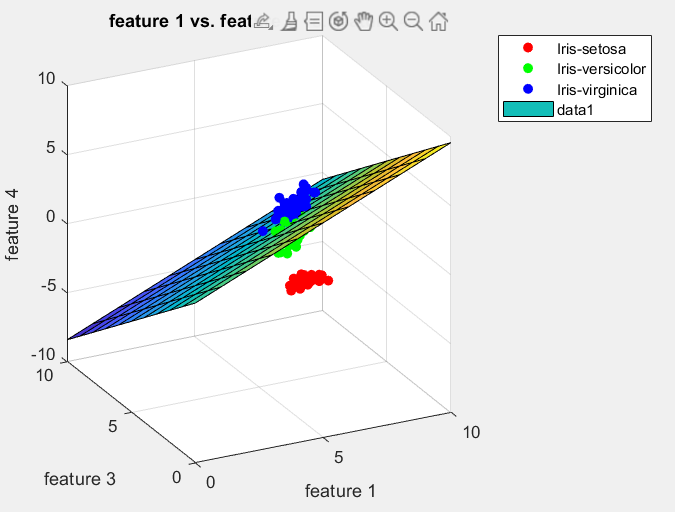
\includegraphics[width=0.4\linewidth]{Fig/Q2_F13.png}
		\qquad\qquad
		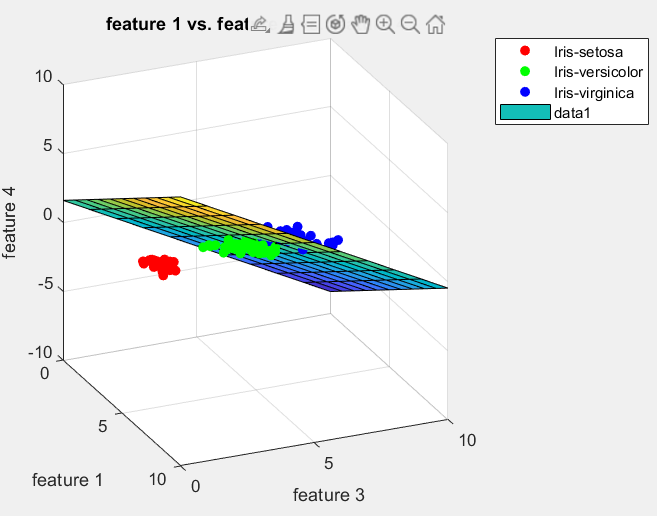
\includegraphics[width=0.4\linewidth]{Fig/Q2_F14.png}
	\end{center}
	Based on the above results, it can be seen that we couldn't even separate training data after 1000 iterations with a 100\% accuracy.\\\\
	The final result of dividing the 3D space into three sections using 2 TLUs for this problem is as follows:
	\begin{center}
		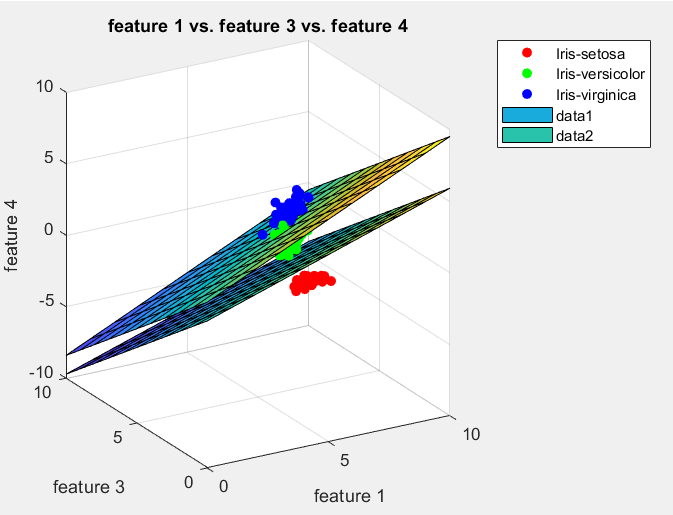
\includegraphics[width=0.4\linewidth]{Fig/Q2_F16.png}
		\qquad\qquad
		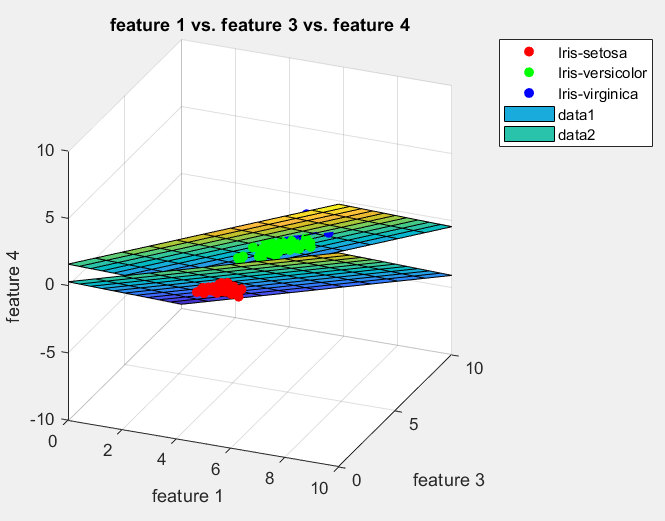
\includegraphics[width=0.4\linewidth]{Fig/Q2_F17.png}
	\end{center}
\end{document}